\section{THIẾT KẾ HỆ THỐNG}\label{sec:thiet_ke}

\subsection{Kiến trúc tổng thể}

Hệ thống gồm năm vùng: Campus chính (Site 100), ba cơ sở phụ (Site 200 Cần Thơ, Site 300 Đà Nẵng, Site 400 Nha Trang), vùng điều khiển SD-WAN (Site 900) và hai mạng truyền tải độc lập là Internet (AS 64511) và MPLS (AS 64512). Từ tháng 10/2026, nhóm bổ sung Site 500 làm chi nhánh mới theo mô hình mạng phẳng để minh họa khả năng mở rộng. Topology logic được trình bày trong Hình~\ref{fig:topology_logic}.

\begin{figure}[H]
    \centering
    \resizebox{\textwidth}{!}{%
    \begin{tikzpicture}[
        font=\scriptsize,
        >=stealth,
        controller/.style={draw=purple!70!black, fill=purple!7, rounded corners, align=center, minimum height=1.2cm, text width=8.0cm},
        transport/.style={draw=black!70, fill=gray!12, rounded corners, align=center, minimum height=0.9cm, text width=3.5cm},
        campus/.style={draw=blue!65!black, fill=blue!5, rounded corners, align=center, minimum height=1.75cm, text width=6.2cm},
        branch/.style={draw=teal!70!black, fill=teal!5, rounded corners, align=center, minimum height=1.55cm, text width=4.4cm},
        newsite/.style={draw=orange!80!black, fill=orange!6, dashed, rounded corners, align=center, minimum height=1.55cm, text width=4.4cm},
        controlLink/.style={draw=purple!75!black, dashed, ->, line width=0.7pt},
        internetLink/.style={draw=blue!75!black, line width=0.9pt},
        mplsLink/.style={draw=orange!85!black, line width=0.9pt}
    ]
        \node[controller] (s900) at (0,3.7) {\textbf{Site 900 -- Control plane SD-WAN}\\
        vManage \texttt{10.9.0.10}; vSmart \texttt{10.9.0.11} (System-IP \texttt{10.9.0.13}); vBond \texttt{10.9.0.12}};

        \node[transport] (internet) at (-7.2,1.35) {\textbf{Internet underlay}\\AS 64511 -- color \texttt{biz-internet}};
        \node[transport] (mpls) at (7.2,1.35) {\textbf{MPLS underlay}\\AS 64512 -- color \texttt{mpls}};

        \node[campus] (s100) at (0,1.35) {\textbf{Site 100 -- Campus chính, AS 65000}\\
        vEdge1/2: \texttt{10.200.100.1/.2}, mỗi edge có Internet và MPLS\\
        ASAv HA -- Core-SW1/2 -- Ryu \texttt{10.1.99.10} điều khiển 6 OVS};

        \node[branch] (s200) at (-7.2,-2.1) {\textbf{Site 200 -- Cần Thơ, AS 65010}\\
        vEdge1 (MPLS), vEdge2 (Internet)\\Brand-FW -- VLAN 60/70};
        \node[branch] (s300) at (-2.4,-2.1) {\textbf{Site 300 -- Đà Nẵng, AS 65020}\\
        vEdge1 (MPLS), vEdge2 (Internet)\\Brand-FW -- VLAN 80/90};
        \node[branch] (s400) at (2.4,-2.1) {\textbf{Site 400 -- Nha Trang, AS 65030}\\
        vEdge1 (MPLS), vEdge2 (Internet)\\Brand-FW -- VLAN 50/60};
        \node[newsite] (s500) at (7.2,-2.1) {\textbf{Site 500 -- chi nhánh mới, AS 65040}\\
        1 vEdge (Internet + MPLS)\\Mạng phẳng \texttt{10.5.1.0/24}};

        \begin{pgfonlayer}{background}
            \draw[internetLink] (internet.east) -- (s100.west);
            \draw[mplsLink] (mpls.west) -- (s100.east);
            \foreach \b in {s200,s300,s400,s500} {
                \draw[internetLink] (internet.south) -- ([xshift=-6mm]\b.north);
                \draw[mplsLink] (mpls.south) -- ([xshift=6mm]\b.north);
            }
            \draw[controlLink] (s900.south) -- (s100.north);
        \end{pgfonlayer}

        \draw[internetLink] (-6.5,-3.5) -- (-5.5,-3.5) node[right, font=\scriptsize] {Internet};
        \draw[mplsLink] (-3.6,-3.5) -- (-2.6,-3.5) node[right, font=\scriptsize] {MPLS};
        \draw[controlLink] (-1.0,-3.5) -- (0.0,-3.5) node[right, font=\scriptsize] {control connection (mọi edge đều có, chỉ vẽ đại diện)};
        \node[font=\scriptsize] at (0,-3.95) {Khung nét đứt: site đang triển khai};
    \end{tikzpicture}%
    }
    \caption{Topology logic của hệ thống tại thời điểm giữa kỳ}
    \label{fig:topology_logic}
\end{figure}

Topology vật lý triển khai trên EVE-NG, gồm đầy đủ thiết bị, cổng kết nối và địa chỉ của từng site, được thể hiện trong Hình~\ref{fig:topology_eve}.

\begin{figure}[!htbp]
    \centering
    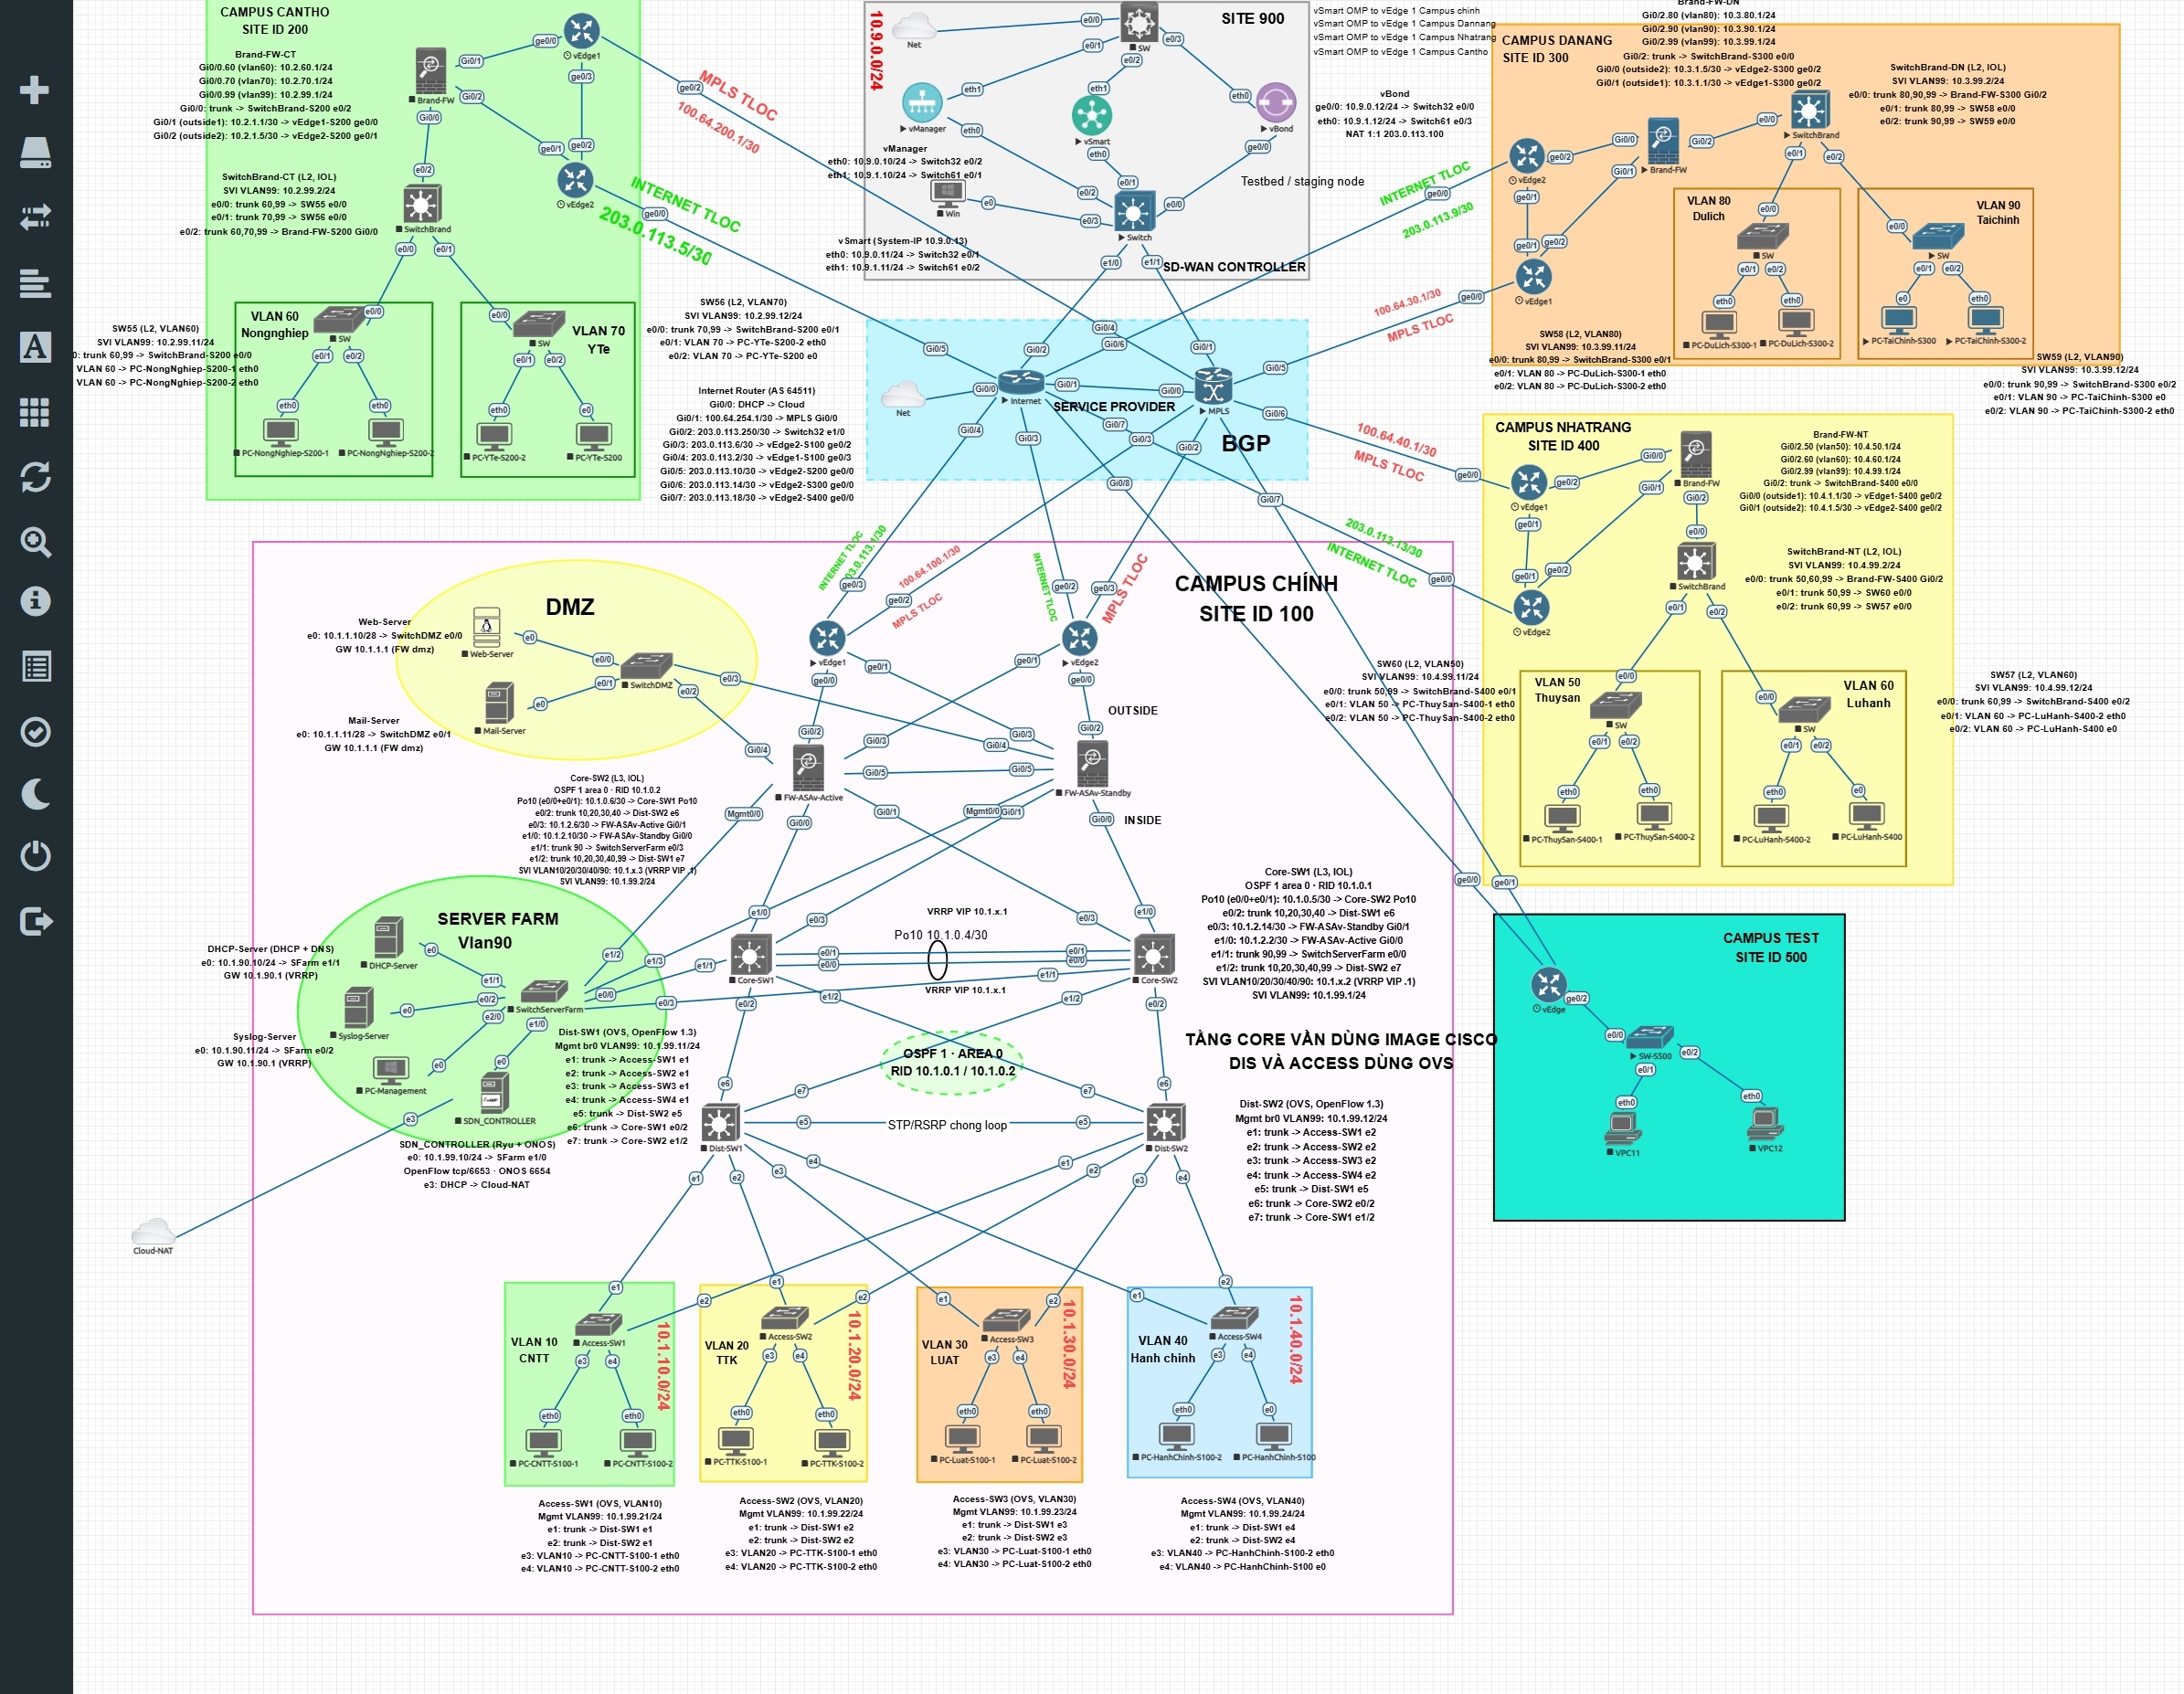
\includegraphics[width=1.0\textwidth]{image/topology.png}
    \caption{Topology vật lý tổng thể của hệ thống trên EVE-NG}
    \label{fig:topology_eve}
\end{figure}

\subsubsection{Campus chính (Site 100)}

Campus chính dùng mô hình ba tầng. Tầng Core gồm Core-SW1/2 (IOL), cung cấp gateway VRRP cho các VLAN và chạy OSPF Area 0 với firewall. Tầng Distribution (Dist-SW1/2) và Access (Access-SW1--4) là sáu Open vSwitch do Ryu điều khiển. Biên mạng là cặp firewall ASAv hoạt động active--standby, nối ra hai vEdge; mỗi vEdge có kết nối tới cả Internet và MPLS. Vùng Server Farm chứa DHCP Server, Syslog Server và SDN Controller; vùng DMZ chứa Web Server và Mail Server. Sơ đồ chi tiết Campus chính được trình bày trong Hình~\ref{fig:campus_chinh}.

\begin{figure}[!htbp]
    \centering
    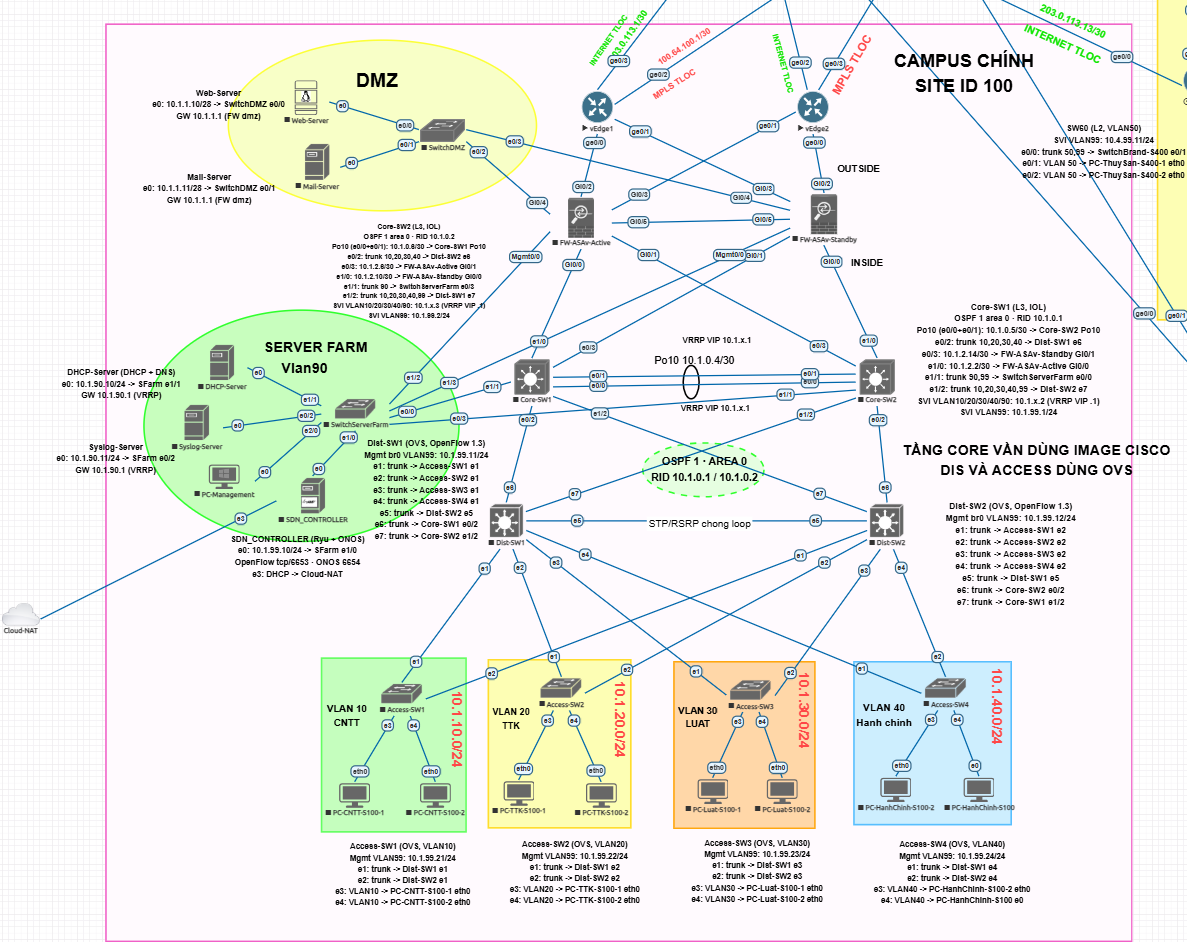
\includegraphics[width=1.0\textwidth]{image/campuschinh.png}
    \caption{Sơ đồ chi tiết Campus chính (Site 100) trên EVE-NG}
    \label{fig:campus_chinh}
\end{figure}


\subsubsection{Các cơ sở phụ (Site 200, 300, 400)}

Ba chi nhánh dùng chung khuôn \textit{Firewall-as-Core}: Brand-FW (ASAv) làm gateway cho các VLAN nghiệp vụ bằng sub-interface và cấp DHCP tại chỗ; SwitchBrand và hai switch phòng ban chỉ làm lớp 2. Mỗi chi nhánh có hai vEdge chia theo transport: vEdge1 nối MPLS, vEdge2 nối Internet. Sơ đồ triển khai của từng chi nhánh được trình bày trong các Hình~\ref{fig:site200}, \ref{fig:site300} và \ref{fig:site400}.

\begin{figure}[!htbp]
    \centering
    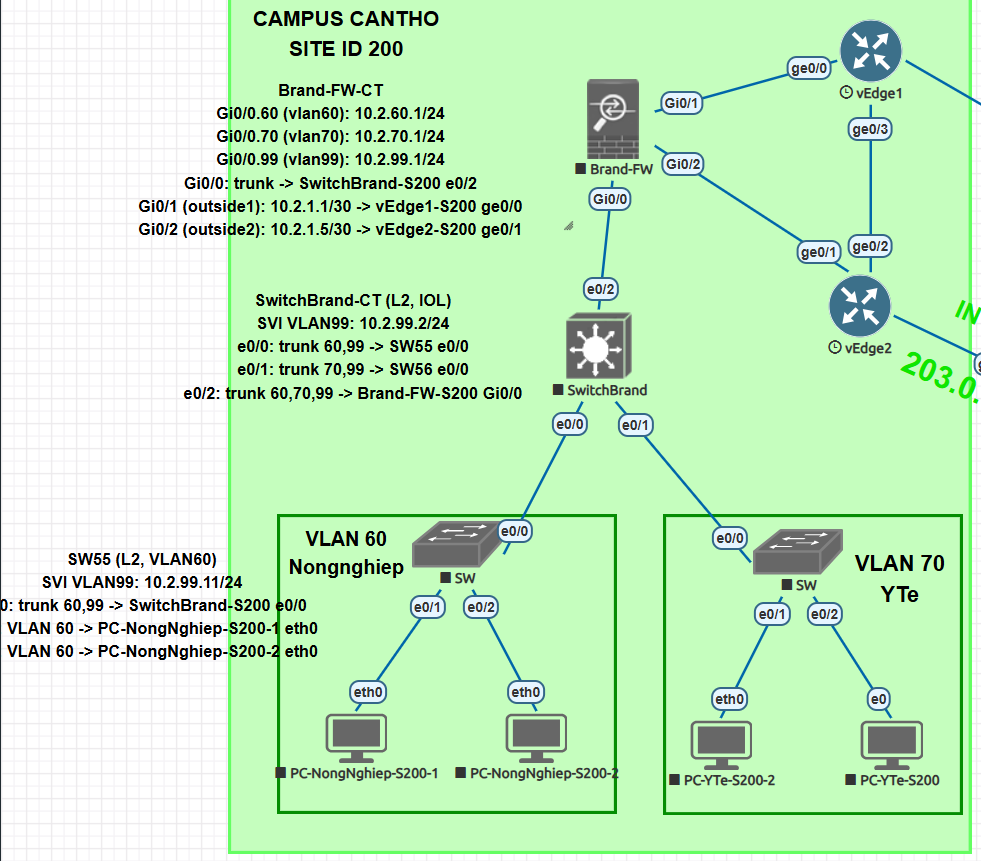
\includegraphics[width=0.75\textwidth]{image/site200.png}
    \caption{Sơ đồ chi nhánh Cần Thơ (Site 200)}
    \label{fig:site200}
\end{figure}

\begin{figure}[!htbp]
    \centering
    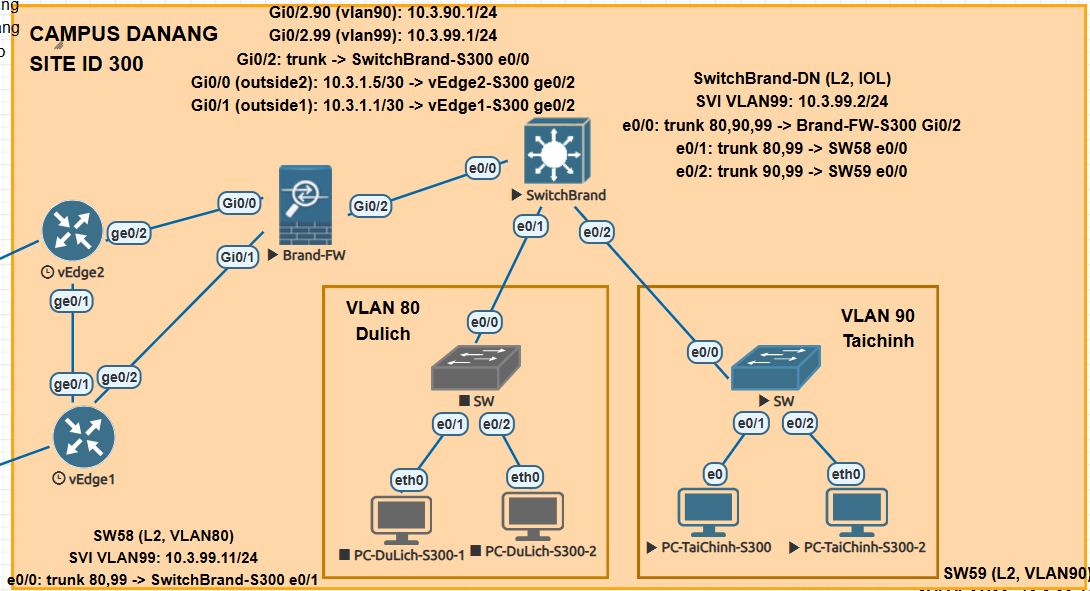
\includegraphics[width=0.80\textwidth]{image/site300.png}
    \caption{Sơ đồ chi nhánh Đà Nẵng (Site 300)}
    \label{fig:site300}
\end{figure}

\begin{figure}[!htbp]
    \centering
    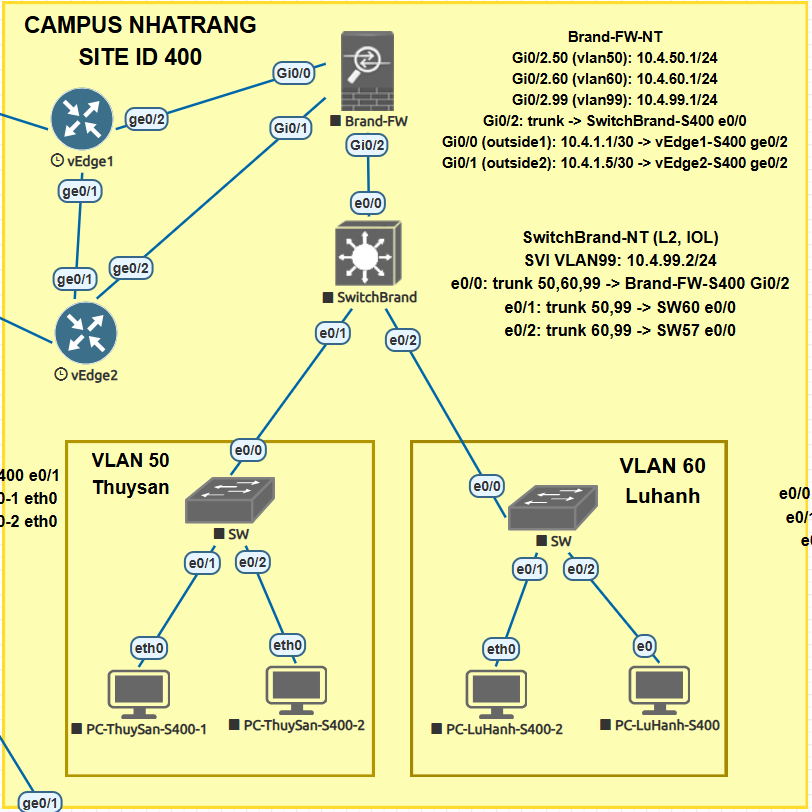
\includegraphics[width=0.80\textwidth]{image/site400.png}
    \caption{Sơ đồ chi nhánh Nha Trang (Site 400)}
    \label{fig:site400}
\end{figure}


\subsubsection{Chi nhánh mạng phẳng (Site 500)}

Site 500 được thiết kế cho cơ sở nhỏ: một vEdge vừa là router WAN, vừa là gateway và DHCP Server cho một subnet duy nhất \texttt{10.5.1.0/24}, không có firewall riêng và không chia VLAN. vEdge này có cả hai transport Internet và MPLS nên vẫn có dự phòng đường truyền, chỉ không có dự phòng thiết bị.

\subsection{Quy hoạch địa chỉ}

Toàn bộ mạng nội bộ dùng dải \texttt{10.0.0.0/8}, trong đó octet thứ hai biểu thị site: 1 (Campus chính), 2, 3, 4, 5 (các chi nhánh) và 9 (controller). Mỗi VLAN dùng subnet /24, gateway là địa chỉ \texttt{.1}, máy chủ dùng \texttt{.10/.11}, dải DHCP cho máy trạm là \texttt{.100--.199}. Liên kết điểm--điểm dùng /30.

\begin{table}[H]
    \centering
    \small
    \caption{Phân hoạch VLAN tại Campus chính}
    \label{tab:vlan_campus}
    \begin{tabularx}{\textwidth}{|c|P{3.2cm}|P{2.8cm}|X|}
        \hline
        \textbf{VLAN} & \textbf{Khu vực} & \textbf{Subnet} & \textbf{Ghi chú} \\
        \hline
        10 & Khoa Công nghệ thông tin & 10.1.10.0/24 & DHCP .100--.199, gateway VRRP .1 \\
        \hline
        20 & Khoa Toán -- Thống kê & 10.1.20.0/24 & DHCP .100--.199, gateway VRRP .1 \\
        \hline
        30 & Khoa Luật & 10.1.30.0/24 & DHCP .100--.199, gateway VRRP .1 \\
        \hline
        40 & Phòng Hành chính & 10.1.40.0/24 & DHCP .100--.199, gateway VRRP .1 \\
        \hline
        90 & Server Farm & 10.1.90.0/24 & DHCP Server .10, Syslog .11 \\
        \hline
        99 & Management và SDN & 10.1.99.0/24 & Controller .10, Dist .11/.12, Access .21--.24 \\
        \hline
        -- & DMZ & 10.1.1.0/28 & Web .10, Mail .11 \\
        \hline
    \end{tabularx}
\end{table}

\begin{table}[H]
    \centering
    \small
    \caption{Phân hoạch mạng tại các cơ sở phụ}
    \label{tab:vlan_chi_nhanh}
    \begin{tabularx}{\textwidth}{|c|c|P{3.2cm}|P{2.8cm}|X|}
        \hline
        \textbf{Site} & \textbf{VLAN} & \textbf{Khu vực} & \textbf{Subnet} & \textbf{Gateway} \\
        \hline
        200 & 60 / 70 & Nông nghiệp / Y tế & 10.2.60.0/24, 10.2.70.0/24 & Brand-FW .1 \\
        \hline
        300 & 80 / 90 & Du lịch / Tài chính & 10.3.80.0/24, 10.3.90.0/24 & Brand-FW .1 \\
        \hline
        400 & 50 / 60 & Thủy sản / Lữ hành & 10.4.50.0/24, 10.4.60.0/24 & Brand-FW .1 \\
        \hline
        500 & -- & Mạng phẳng & 10.5.1.0/24 & vEdge .1 \\
        \hline
    \end{tabularx}
\end{table}

\subsection{Quy hoạch SD-WAN}

System-IP là địa chỉ định danh vEdge trong OMP, có dạng \texttt{10.200.<site>.x}; với site có số lớn hơn 255, octet được rút gọn (300 thành 30, 400 thành 40, 500 thành 50, 900 thành 90). Underlay dùng eBGP giữa vEdge (CE) và router nhà cung cấp (PE); router PE quảng bá default route xuống vEdge. Các controller SD-WAN (vManage, vSmart, vBond) đặt tại Site 900, dùng chung subnet \texttt{10.9.0.0/24} và kết nối tới cả hai mạng truyền tải (Hình~\ref{fig:site900}).

\begin{figure}[!htbp]
    \centering
    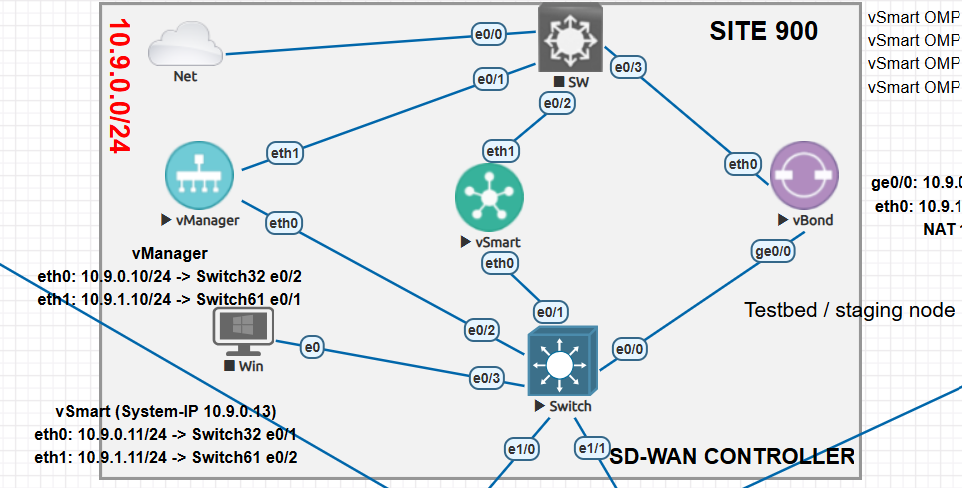
\includegraphics[width=0.75\textwidth]{image/site900.png}
    \caption{Vùng điều khiển SD-WAN (Site 900)}
    \label{fig:site900}
\end{figure}


\begin{table}[H]
    \centering
    \scriptsize
    \caption{System-IP, ASN và TLOC của các vEdge}
    \label{tab:system_ip}
    \begin{tabularx}{\textwidth}{|c|P{2.0cm}|c|P{2.3cm}|c|P{2.6cm}|X|}
        \hline
        \textbf{Site} & \textbf{Thiết bị} & \textbf{Node} & \textbf{System-IP} & \textbf{ASN} & \textbf{TLOC Internet} & \textbf{TLOC MPLS} \\
        \hline
        100 & vEdge1-S100 & 28 & 10.200.100.1 & 65000 & 203.0.113.1/30 & 100.64.100.1/30 \\
        \hline
        100 & vEdge2-S100 & 6 & 10.200.100.2 & 65000 & 203.0.113.5/30 & 100.64.100.5/30 \\
        \hline
        200 & vEdge1-S200 & 29 & 10.200.200.1 & 65010 & -- & 100.64.200.1/30 \\
        \hline
        200 & vEdge2-S200 & 42 & 10.200.200.2 & 65010 & 203.0.113.9/30 & -- \\
        \hline
        300 & vEdge1-S300 & 30 & 10.200.30.1 & 65020 & -- & 100.64.30.1/30 \\
        \hline
        300 & vEdge2-S300 & 40 & 10.200.30.2 & 65020 & 203.0.113.13/30 & -- \\
        \hline
        400 & vEdge1-S400 & 31 & 10.200.40.1 & 65030 & -- & 100.64.40.1/30 \\
        \hline
        400 & vEdge2-S400 & 41 & 10.200.40.2 & 65030 & 203.0.113.17/30 & -- \\
        \hline
        500 & vEdge-S500 & 65 & 10.200.50.1 & 65040 & 203.0.113.21/30 & 100.64.50.1/30 \\
        \hline
    \end{tabularx}
\end{table}

\subsection{Các quyết định thiết kế chính}

\begin{itemize}
    \item \textbf{Control plane SDN đi trong VLAN 99:} kênh OpenFlow dùng chính các uplink sẵn có thay vì mạng điều khiển riêng. Đường VLAN 99 được cắt tỉa thành cây không vòng lặp để controller luôn tới được switch trước khi flow được cài.
    \item \textbf{Core dùng IOL thay vIOS-L2:} image vIOS-L2 bị treo CPU khi có broadcast từ OVS và nạp cấu hình không ổn định; IOL hỗ trợ đầy đủ SVI, VRRP và OSPF.
    \item \textbf{Firewall-as-Core tại chi nhánh:} Brand-FW vừa là gateway vừa cấp DHCP, giảm số thiết bị và giúp chi nhánh vẫn cấp địa chỉ khi WAN gián đoạn.
    \item \textbf{Underlay BGP thay OSPF:} mô phỏng đúng quan hệ khách hàng--nhà cung cấp; vEdge học default route động từ cả hai transport.
    \item \textbf{Site 500 mạng phẳng:} minh họa mô hình chi nhánh nhỏ chi phí thấp, chứng minh việc thêm site mới chỉ cần cấp Site ID, System-IP, chứng thư và cập nhật danh sách site trong chính sách.
\end{itemize}

\subsection{Phương án dự phòng}

Dự phòng được bố trí ở từng tầng để một sự cố đơn lẻ không làm gián đoạn toàn bộ dịch vụ. Bảng~\ref{tab:du_phong} tổng hợp cơ chế dự phòng và các điểm lỗi đơn còn tồn tại trong thiết kế hiện tại.

\begin{table}[H]
    \centering
    \small
    \caption{Cơ chế dự phòng theo từng tầng}
    \label{tab:du_phong}
    \begin{tabularx}{\textwidth}{|P{3.0cm}|X|P{3.6cm}|}
        \hline
        \textbf{Tầng / thành phần} & \textbf{Cơ chế dự phòng} & \textbf{Ghi chú} \\
        \hline
        Gateway Campus chính & VRRP giữa Core-SW1 và Core-SW2 & Máy trạm giữ nguyên gateway .1 \\
        \hline
        Firewall Campus chính & Cặp ASAv active--standby, đồng bộ cấu hình & Kiểm thử failover ở giai đoạn cuối \\
        \hline
        WAN Campus chính & Hai vEdge, mỗi vEdge có cả Internet và MPLS & Dự phòng cả thiết bị và đường truyền \\
        \hline
        WAN chi nhánh 200--400 & Hai vEdge, mỗi vEdge một transport & Mất một vEdge vẫn còn transport kia \\
        \hline
        WAN Site 500 & Một vEdge với hai transport & Chỉ dự phòng đường truyền \\
        \hline
        Đường hầm SD-WAN & BFD phát hiện mất kết nối, AAR chuyển đường theo SLA & Chu kỳ đo ảnh hưởng thời gian chuyển \\
        \hline
        Controller SDN & Một controller Ryu & Điểm lỗi đơn; OVS giữ flow đã cài \\
        \hline
        Controller SD-WAN & Một vManage, một vSmart, một vBond & Data plane vẫn chạy trong thời gian ân hạn \\
        \hline
    \end{tabularx}
\end{table}

\subsection{Luồng lưu lượng điển hình}

Để minh họa cách các thành phần phối hợp, xét một máy trạm VLAN 60 tại Site 200 truy cập Web Server trong DMZ của Campus chính. Gói tin đi qua switch phòng ban và SwitchBrand tới Brand-FW, nơi đóng vai trò gateway và kiểm tra ACL. Brand-FW chuyển gói tới vEdge chi nhánh trong service VPN 1; vEdge tra bảng tuyến học từ OMP, chọn đường hầm IPsec tới vEdge của Site 100 theo chính sách AAR, rồi đóng gói và gửi qua transport tương ứng. Tại Site 100, vEdge giải đóng gói và chuyển gói tới cặp ASAv; firewall chỉ cho phép các dịch vụ đã khai báo đi vào DMZ. Chiều về đi theo đường ngược lại. Trong suốt quá trình, vSmart không nằm trên đường dữ liệu mà chỉ phân phối tuyến và chính sách cho các vEdge.
